\section{Avbrudd}
\label{sec:avbrudd}
Eksterne avbrytelser refererer til situasjoner hvor eksterne hendelser forstyrrer pågående aktiviteter \citep{Harr07}. Da mange arbeidsaktiviteter er kognitive, altså krever tenkning, problemløsing og evnen til å forutse og ta beslutninger, argumenterer \citet{Rogers94} for at det kreves en forståelse for hvordan disse aktivitetene utføres for å kunne designe datasystemer som kan støtte både kognitive aktiviteter og sosial interaksjon.

\tikzstyle{mybox} = [draw=black, fill=white, very thick,
    rectangle, inner sep=10pt, inner ysep=20pt, rounded corners]
\tikzstyle{fancytitle} =[fill=black, text=white]
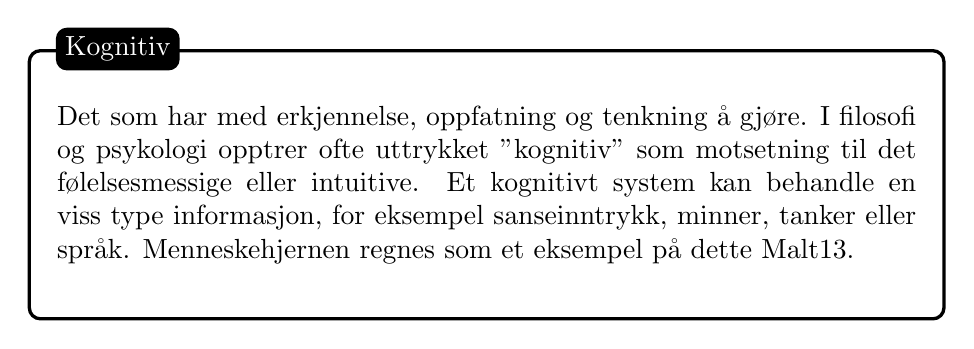
\begin{tikzpicture}
\node [mybox] (box){%
    \begin{minipage}{0.9\textwidth}
     Det som har med erkjennelse, oppfatning og tenkning å gjøre. I filosofi og psykologi opptrer ofte uttrykket $"$kognitiv$"$ som motsetning til det følelsesmessige eller intuitive. Et kognitivt system kan behandle en viss type informasjon, for eksempel sanseinntrykk, minner, tanker eller språk. Menneskehjernen regnes som et eksempel på dette \citep{Malt13}.
    \end{minipage}
};
\node[fancytitle, rounded corners, right=10pt] at (box.north west) {Kognitiv};
\end{tikzpicture}%

\noindent
Det skilles normalt mellom langtids- og korttidsminne. Den passive kunnskapen man besitter ligger i langtidsminnet, for eksempel medisinske fakta eller viktige datoer. Korttidsminnet, eller arbeidsminnet, er den bevisste delen av minnet som aktivt behandler informasjon. Arbeidsminnet har begrenset kapasitet og varighet og lar seg raskt forstyrre av distraksjoner og avbrytelser \citep{Parker00}. 

\noindent
Stadige endringer i omgivelser og informasjonsflyt resulterer i en kontinuerlig omprioritering av hvilke oppgaver som skal utføres når. Dette kombinert med avbrytelser fra omgivelsene kan resultere i en kognitiv belastning som kan hemme oppmerksomheten \citep{Ebright10}, og studier har vist at feil og ineffektivitet kan være et resultat av at kognitiv kapasitet overskrides \citep{Parker00}. Kunnskap om menneskets hukommelse hevdes å være nøkkelen til å forstå hvilke krav som bør settes til teknologi brukt i slike omgivelser.

\subsection{Dualiteten ved avbrudd}
\label{sec:dualitet}
\citet{Grundgeiger09} skiller mellom gode og dårlige avbrudd, og hevder disse må sees i sammenheng med hvilke effekter de har. Eksempler på positive effekter er øyeblikkelig kommunikasjon og tilgang til viktig informasjon. Avbryter opplever å få en umiddelbar bekreftelse på at informasjonen er mottatt og kan dermed avlaste arbeidsminnet, mens den som blir avbrutt kan oppleve negative effekter, som overbelastet kognitiv kapasitet, forsinkelse i eget arbeid, stress og frustrasjon. Avbruddet kan også ha en positiv effekt dersom den avbrutte mottar ønsket informasjon.

\subsection{Avbruddshåndtering}
\label{sec:håndtering}
Gitt dualiteten ved avbrudd kan avbruddshåndtering sies å ha to mål: (1) redusere de negative effektene og (2) utnytte de positive effektene ved avbrudd. \citet{Grandhi10} gir fire teknikker for avbruddshåndtering:
\begin{enumerate}        
\item Forebygging - bruk av funksjoner som forebygger eller blokkerer innkommende avbrytelser. Dette kan enkelt gjøres ved å for eksempel skru av mobilen for en periode. En annen strategi er å kontrollere timingen til avbruddet eller å kun tillate avbrytelser som er relevant for den oppgaven man utfører.

\item Fraråding - bruk av funksjoner som fraråder avbrytelser. Dette skjer ofte ved at man gir informasjon til avbryter om tilgjengeligheten til den man ønsker å avbryte. 

\item Modifiserte varslinger - bruk av funksjoner som modifiserer hvordan individer varsles om innkommende anrop. Ved bruk av ulike modaliteter som lyd, vibrasjon og lys, kan man minimere interferensen mellom perseptuelle og kognitive prosesser involvert i avbruddshåndtering og oppgaveytelse \citep{Harr07}.

\item Forhåndsvisning - bruk av funksjoner som gir informasjon om selve avbrytelsen som den avbrutte selv kan reflektere over.   
\end{enumerate}

